\section{if else语句}

\begin{frame}[fragile]\ft{\secname}
\begin{lstlisting}
if (condition)
  statement1
else
  statement2
\end{lstlisting} \pause 
\begin{itemize}
\item  若满足条件(condition为真),则执行statement1;
\item[]若不满足条件(condition为假),则执行statement2。\\[0.1in]
\item 语句可以是简单语句或复合语句。\\[0.1in]
\item 注意缩进。
\end{itemize}
\end{frame}

\begin{frame}[fragile]\ft{\secname}
若if和else之间有多条语句,\red{必须}使用花括号。
\begin{lstlisting}
// wrong structure
if (x > 0)
  printf("Incrementing x:\n");
  x++;
else
  printf("x <= 0\n");
\end{lstlisting}\pause
\begin{itemize}
\item  编译器会把printf语句看做if的一部分,而把x++;看做是一条单独的语句,而不是if的一部分。\\[0.1in]
\item 然后认为else没有对应的if,于是报错。
\end{itemize}
\end{frame}

\begin{frame}[fragile]\ft{\secname}
\begin{lstlisting}
// right structure
if (x > 0){
  printf("Incrementing x:\n");
  x++;
}	
else
  printf("x <= 0\n");
\end{lstlisting}
\end{frame}



\begin{frame}[fragile]\ft{\secname}
\begin{figure}
\centering
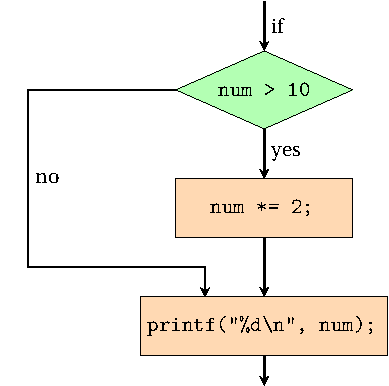
\includegraphics[width=3in]{ch07/images/if.pdf}
\end{figure}

\end{frame}


\begin{frame}[fragile]\ft{\secname}
\begin{figure}
\centering
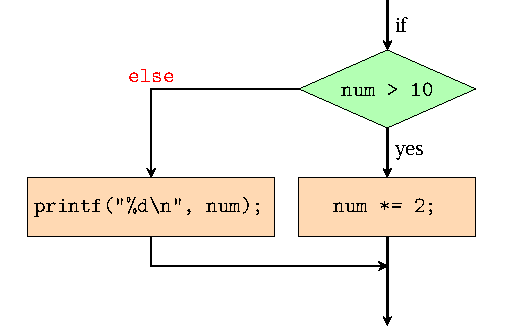
\includegraphics[width=4in]{ch07/images/if1.pdf}
\end{figure}

\end{frame}



\begin{frame}[fragile]\ft{getchar与putchar函数}
\begin{itemize}
\item 
函数getchar没有参数,返回来自输入设备的下一个字符。 \\[0.1in]

\begin{minipage}{0.3\textwidth}
\begin{lstlisting}[backgroundcolor=\color{red!20},]
ch = getchar();
\end{lstlisting} 
\end{minipage}
$~~ \Longleftrightarrow~~$
\begin{minipage}{0.4\textwidth}
\begin{lstlisting}[backgroundcolor=\color{red!20},]
scanf("%c", &ch);
\end{lstlisting} 
\end{minipage} \vspace{0.1in}

\item 
函数putchar打印它的参数。 \\[0.1in]

\begin{minipage}{0.35\textwidth}
\begin{lstlisting}[backgroundcolor=\color{red!20},]
putchar(ch);
\end{lstlisting} 
\end{minipage}
$~~\blue \Longleftrightarrow~~$
\begin{minipage}{0.4\textwidth}
\begin{lstlisting}[backgroundcolor=\color{red!20},]
printf("%c", ch);
\end{lstlisting} 
\end{minipage}
\end{itemize}
\end{frame}

\begin{frame}[fragile]\ft{getchar与putchar函数}
\begin{itemize}
\item 
只处理字符,比函数scanf和printf更快更简洁。\\[0.1in]
\item
不需要格式说明符。\\[0.1in]
\item
在stdio.h中定义。事实上,它们只是宏定义,不是真正的函数。
\end{itemize}
\end{frame}

\begin{frame}[fragile]\ft{getchar与putchar函数}
  \begin{minipage}{0.65\textwidth}
\lstinputlisting[language=c,numbers=left,frame=single]{ch07/code/cypher1.c}    
  \end{minipage}~~~\pause 
  \begin{minipage}{0.3\textwidth}
\begin{lstlisting}[backgroundcolor=\color{blue!20}]
Hello World
Ifmmp Xpsme
\end{lstlisting}    
  \end{minipage}

\end{frame}


\begin{frame}[fragile]\ft{getchar与putchar函数}
\begin{lstlisting}[language=c,frame=single]
ch = getchar();
while (ch != '\n') {
  ...
  ch = getchar();
}
\end{lstlisting} 
可改写为
\begin{lstlisting}[language=c,frame=single]
while ((ch = getchar()) != '\n') {
  ...   
}
\end{lstlisting} \pause \vspace{0.1in}

这体现了典型的C编程风格:将两个动作合并为一个表达式。
\end{frame}

\begin{frame}[fragile]\ft{getchar与putchar函数}
更建议写成
\begin{lstlisting}[language=c,frame=single]
while (
       (ch = getchar()) 
           != '\n') {
  ...   
}
\end{lstlisting}
\end{frame}

\begin{frame}[fragile]\ft{getchar与putchar函数}

\begin{itemize}
\item 两个动作:将某个值赋给 \lstinline|ch|,并将这个值与换行符作比较。\\[0.1in]
\item 圆括号使 \lstinline|ch = getchar()| 称为 \lstinline|!=| 的左操作数。\\[0.1in]
\item 先调用函数 \lstinline|getchar|,将其返回值赋给 \lstinline|ch|。而\blue{赋值表达式的值等于左操作数的值},故 \lstinline| ch = getchar()| 的值等于 \lstinline|ch| 的值。\\[0.1in]
\item 最后将 \lstinline|ch| 与换行符做比较。
\end{itemize}
\end{frame}

\begin{frame}[fragile]\ft{getchar与putchar函数}
 圆括号是必须的。若写成
\begin{lstlisting}
while ( ch = getchar() != '\n') {
  ...   
}
\end{lstlisting}
首先会计算表达式 \lstinline|getchar() != '\n'|,其值为0或1,然后这个值被赋给 \lstinline|ch|。于是 \lstinline|ch| 将会被赋为0或1,而不是 \lstinline|getchar| 的返回值。
\end{frame}

\begin{frame}[fragile]\ft{ctype.h:字符函数}
\lstinputlisting[language=c,numbers=left,frame=single]{ch07/code/cypher2.c}
\end{frame}

\begin{frame}[fragile]\ft{ctype.h:字符函数}
\begin{lstlisting}[backgroundcolor=\color{red!10}]
Look! It's a programmer!
Mppl! Ju't b qsphsbnnfs!
\end{lstlisting}
\end{frame}

\begin{frame}[fragile]\ft{ctype.h:字符函数}
\begin{table}
\centering
\caption{字符判断函数}
\begin{tabular}{p{2cm}|p{8cm}}\hline
函数名&为如下参数时,返回值为真\\\hline\hline
\lstinline|isalnum| & 字母或数字\\[0.1in] 
\lstinline|isalpha| & 字母 \\[0.1in] 
\lstinline|isblank| & 标准空白字符(空格、水平制表符或换行符) \\[0.1in] 
\lstinline|iscntrl| & 控制符,如Ctrl+B \\[0.1in] 
\lstinline|isdigit| & 阿拉伯数字 \\[0.1in]
\lstinline|isgraph| & 除空格字符之外的所有可打印字符 \\\hline
\end{tabular}
\end{table}
\end{frame}

\begin{frame}[fragile]\ft{ctype.h:字符函数}
\begin{table}
\centering
\caption{字符判断函数}
\begin{tabular}{p{2cm}|p{8cm}}\hline
函数名&为如下参数时,返回值为真\\\hline\hline
\lstinline|islower| & 小写字母\\[0.1in]
\lstinline|isprint| & 可打印字符 \\[0.1in]
\lstinline|ispunct| & 标点符号 \\[0.1in] 
\lstinline|isspace| & 空白字符:空格、换行、水平(垂直)制表符、回车 \\[0.1in] 
\lstinline|isupper| & 大写字母 \\[0.1in] 
\lstinline|isxdigit| & 十六进制数字字符 \\\hline
\end{tabular}
\end{table}
\end{frame}

\begin{frame}[fragile]\ft{ctype.h:字符函数}
\begin{table}
\centering
\caption{字符映射函数}
\begin{tabular}{p{2cm}|p{8cm}}\hline
函数名&动作\\\hline\hline 
\lstinline|tolower| & 若参数为大写字母,则返回相应的小写字母;否则返回原始参数\\[0.1in]
\lstinline|toupper| & 若参数为小写字母,则返回相应的大写字母;否则返回原始参数 \\\hline
\end{tabular}
\end{table}
\end{frame}

\begin{frame}[fragile]\ft{ctype.h:字符函数}
字符映射函数不改变原始参数,只返回改变后的值。也就是说,以下语句不改变ch的值
\begin{lstlisting}
tolower(ch);
\end{lstlisting}
若想改变ch,可使用
\begin{lstlisting}
ch = tolower(ch);
\end{lstlisting}
\end{frame}

\begin{frame}[fragile]\ft{多重选择else if}
\begin{li}
某电力公司的费率如下:
\begin{table}
\centering
\begin{tabular}{r|l}\hline
第一个360kwh& \$0.12589/kwh\\[0.1in]
下一个320kwh& \$0.17901/kwh\\[0.1in]
超过680kwh & \$0.20971/kwh
\\\hline
\end{tabular}
\end{table}
编制程序,计算你的用电费用。
\end{li}
\end{frame}


\begin{frame}[fragile,allowframebreaks]\ft{多重选择else if}
\lstinputlisting
{ch07/code/electric.c}
\end{frame}



\begin{frame}[fragile]\ft{多重选择else if}
\begin{lstlisting}
Please enter the kwh used.
580
The charge for 580.0 kwh is $84.70.
\end{lstlisting}
\end{frame}


\begin{frame}[fragile]\ft{多重选择else if}
\begin{figure}
\centering
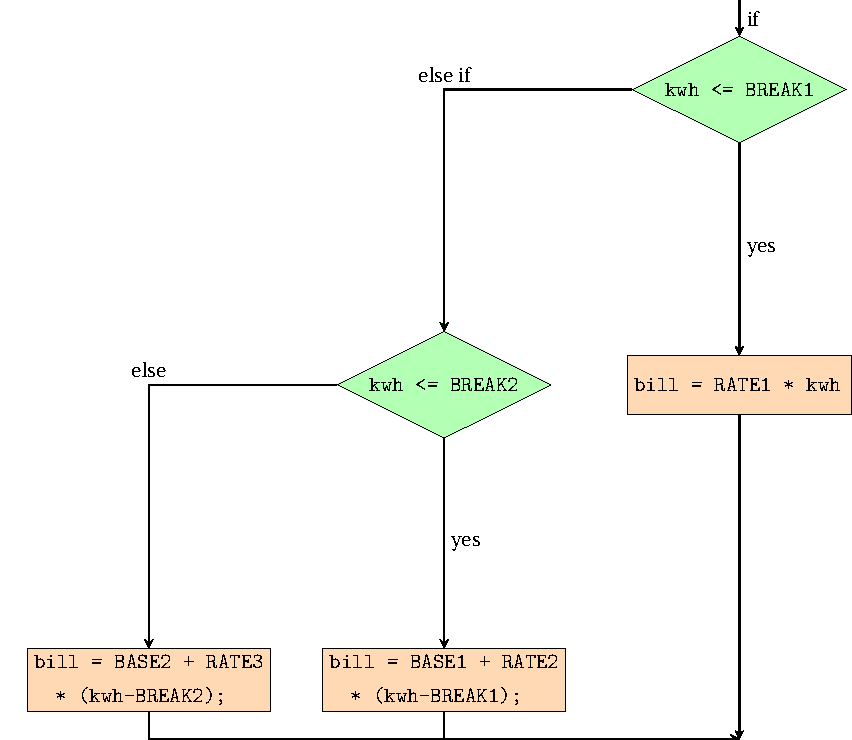
\includegraphics[width=3in]{ch07/images/elseif.pdf}
\end{figure}

\end{frame}


\begin{frame}[fragile]\ft{多重选择else if}
\begin{lstlisting}
if (kwh <= BREAK1)
  bill = RATE1 * kwh;
else if (kwh <= BREAK2)
  bill = BASE1 + RATE2 * (kwh - BREAK1);
else
  bill = BASE2 + RATE3 * (kwh - BREAK2);
\end{lstlisting}
等价于
\begin{lstlisting}
if (kwh <= BREAK1)
  bill = RATE1 * kwh;
else 
  if (kwh <= BREAK2)
    bill = BASE1 + RATE2 * (kwh - BREAK1);
  else
    bill = BASE2 + RATE3 * (kwh - BREAK2);
\end{lstlisting}
\end{frame}


\begin{frame}[fragile]\ft{多重选择else if}
\begin{itemize}
\item
第二种形式是if else语句的嵌套。因\blue{整个if else结构是一条语句},故第一个else后面不需要用花括号。\\[0.1in]
\item 
虽然两种形式完全等价,但建议采用第一种形式,它可以更清晰地展示出有三种选择。
\end{itemize}
\end{frame}


\begin{frame}[fragile]\ft{多重选择else if}
可以把多个所需的else if语句连成一串使用。
\begin{lstlisting}
if (score < 1000)
  bonus = 0;
else if (score < 1500)
  bonus = 1;
else if (score < 2000)
  bonus = 2;
else if (score < 2500)
  bonus = 3;
else
  bonus = 4;    
\end{lstlisting}
\blue{编译器对嵌套层数有限制,C99标准要求编译器最少支持127层嵌套。}
\end{frame}

\begin{frame}[fragile]\ft{else与if的配对}
\lstinputlisting[language=c,numbers=left,frame=single]{ch07/code/elseif.c}
\end{frame}

\begin{frame}[fragile]\ft{else与if的配对}
\begin{lstlisting}
Enter an integer: 5
\end{lstlisting} \pause
 
\begin{lstlisting}
Enter an integer: 10
You're close!
\end{lstlisting} \pause 

\begin{lstlisting}
Enter an integer: 15
Sorry, you loose a turn!
\end{lstlisting}
\end{frame}

\begin{frame}[fragile]\ft{else与if的配对}
\begin{block}{规则}
如果没有花括号,else与和它最近的一个if相匹配。
\end{block}
\end{frame}

\begin{frame}[fragile]\ft{else与if的配对}
上例最好改写为
\begin{lstlisting}{ch07/code/elseif.c}
  if (number > 6)
    if (number < 12)
      printf("You're close!\n");
    else
      printf("Sorry, you loose a turn!\n");
\end{lstlisting}
\end{frame}

\begin{frame}[fragile]\ft{else与if的配对}
若真的希望else和第一个if匹配,请写成
\begin{lstlisting}{ch07/code/elseif.c}
  if (number > 6) {
    if (number < 12)
      printf("You're close!\n");
  }
  else
    printf("Sorry, you loose a turn!\n");
\end{lstlisting}
\end{frame}

\begin{frame}[fragile]\ft{多层嵌套的分支结构}
  \begin{li}
    编写程序,由用户输入一个整数,然后判断其是否为质数。如果不是质数,请求出其公约数。
  \end{li}
\end{frame}

\begin{frame}[fragile,allowframebreaks]\ft{多层嵌套的分支结构}
\lstinputlisting
{ch07/code/divisors.c}
\end{frame}


\begin{frame}[fragile,allowframebreaks]\ft{多层嵌套的分支结构}
\begin{lstlisting}
Enter an integer (Enter q to quit).
36
36 is divisible by 2 and 18.
36 is divisible by 3 and 12.
36 is divisible by 4 and 9.
36 is divisible by 6.
Enter another integer (Enter q to quit).
149
149 is prime.
Enter another integer (Enter q to quit).
30777
30777 is divisible by 3 and 10259.
Enter another integer (Enter q to quit).
q
Bye.
\end{lstlisting}
\end{frame}

% \begin{frame}[fragile]\ft{小结}
% \begin{itemize}
% \item 关键字:if、else \\[0.1in]
% \item 以下各种形式中,语句部分可以是一条简单语句,也可以是复合语句。
% \end{itemize}
% \end{frame}

% \begin{frame}[fragile]\ft{小结}
% \begin{lstlisting}[title=形式1]
% if (condition)
%   statement
% \end{lstlisting}
% \end{frame}

% \begin{frame}[fragile]\ft{小结}
% \begin{lstlisting}[title=形式2]
% if (condition)
%   statement1
% else
%   statement2  
% \end{lstlisting}
% \end{frame}

% \begin{frame}[fragile]\ft{小结}
% \begin{lstlisting}[title=形式3]
% if (condition1)
%   statement1
% else if (condition2)
%   statement2  
% else
%   statement3
% \end{lstlisting}
% \end{frame}

